\documentclass[paper=a4, fontsize=11pt]{scrartcl}
\usepackage{amsmath,amsfonts,amsthm}
\usepackage{sectsty}
\usepackage{fourier} % Use the Adobe Utopia font for the document - comment this line to return to the LaTeX default
\usepackage[english]{babel}
\allsectionsfont{ \normalfont\scshape}
\usepackage{fancyhdr}
\usepackage{float}
\usepackage{graphicx}
\usepackage{listings}
\pagestyle{fancyplain}

\fancyhead{} % No page header - if you want one, create it in the same way as the footers below
\fancyfoot[L]{} % Empty left footer
\fancyfoot[C]{} % Empty center footer
\fancyfoot[R]{\thepage} % Page numbering for right footer
\renewcommand{\headrulewidth}{0pt} % Remove header underlines
\renewcommand{\footrulewidth}{0pt} % Remove footer underlines
\renewcommand\floatpagefraction{.9}
\setlength{\headheight}{13.6pt} % Customize the height of the header
\numberwithin{equation}{section} % Number equations within sections (i.e. 1.1, 1.2, 2.1, 2.2 instead of 1, 2, 3, 4)
\numberwithin{figure}{section} % Number figures within sections (i.e. 1.1, 1.2, 2.1, 2.2 instead of 1, 2, 3, 4)
\numberwithin{table}{section} % Number tables within sections (i.e. 1.1, 1.2, 2.1, 2.2 instead of 1, 2, 3, 4)
\setlength\parindent{0pt} % Removes all indentation from paragraphs - comment this line for an assignment with lots of text
\renewcommand{\thesubsection}{\thesection\alph{subsection}}


\setlength\floatsep{1.25\baselineskip plus 2pt minus 2pt}
\setlength\textfloatsep{1.25\baselineskip plus 2pt minus 2pt}



%----------------------------------------------------------------------------------------
%	TITLE SECTION
%----------------------------------------------------------------------------------------

\newcommand{\horrule}[1]{\rule{\linewidth}{#1}} % Create horizontal rule command with 1 argument of height
\title{	
\normalfont \normalsize 
\textsc{Yale-NUS College} \\ [20pt]
\textsc{YID3202C : Data Analysis in Environmental Studies } \\ [25pt] % Your university, school and/or department name(s)
\horrule{0.5pt} \\[0.4cm] % Thin top horizontal rule
\huge Problem Set One \\ % The assignment title
\horrule{2pt} \\[0.5cm] % Thick bottom horizontal rule
}

\author{Jake Goh Si Yuan} % Your name

\date{\normalsize October 16, 2016} % Today's date or a custom date


\begin{document}

\maketitle % Print the title
\section{Fitting Trends Over the Entire Data Series}
\subsection{}
The average increase of $CO_2$ concentration per year from the linear regression model of $CO_2$ concentration with time(with 1958 as origin) is 1.520, and the average increase per decade is 15.20.

\subsection{}
Taking the time data, with origin 0 set as year 1958 and with year 2016 represented as 58, we will arrive at a nominal start-point of 307ppm and endpoint of 395.16ppm\\

The start-point of the data is 315.71ppm or 8.71ppm higher than trend-predicted, and the end-point is 402.25ppm or 7.19ppm higher.
\subsection{}

The standard deviation of the data-misfit residual, or the residual standard error, is 3.871 on 700 degrees of freedom. The F variance ratio, or statistic, is 30880.
\pagebreak
\subsection{}
\begin{figure}[htp]
	\centering
	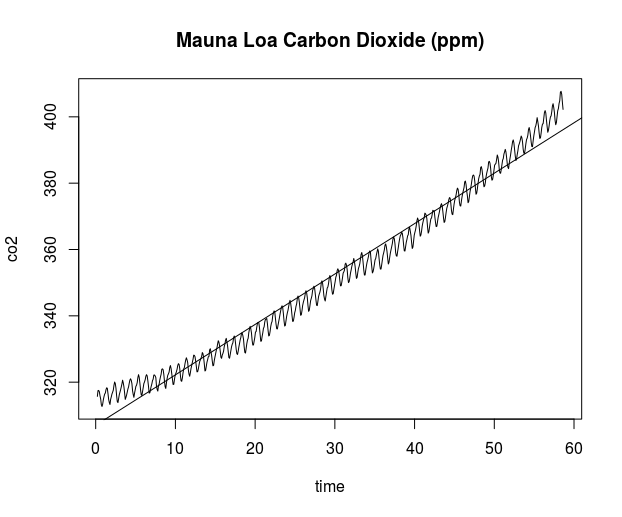
\includegraphics[width=0.7\textwidth, clip]{q1aTime.png} 
	\caption{Linear regression of time(with 1958 as origin) and Mauna Loa Carbon Dioxide}
\end{figure}

The data does not seem to follow strictly to a straight line, in fact, it appears to be have an exponential trend with a small enough exponent that it takes on pseudo-linear characteristics.\\

Also, the linear prediction fails to take into account the saw-tooth motion that the data is taking, or the trend within the trend.

\subsection{}

The predicted start-point for the quadratic model is 314.2ppm, as compared to the actual start-point of 315.71ppm, with a difference of -1.51ppm.

The predicted end-point is 401.89ppm, as compared to the actual end-point of 402.25ppm, with a difference of -0.36ppm.

\subsection{}
The predicted yearly increase at the start-point of the quadratic model is 0.8055ppm, and at the end-point it is 
2.235ppm.

\subsection{}
The standard deviation of the data-misfit residual, or the residual standard error, is 2.209 on 699 degrees of freedom. The F variance ratio, or statistic, is 48160.

\subsection{}

\begin{figure}[htp]
	\centering
	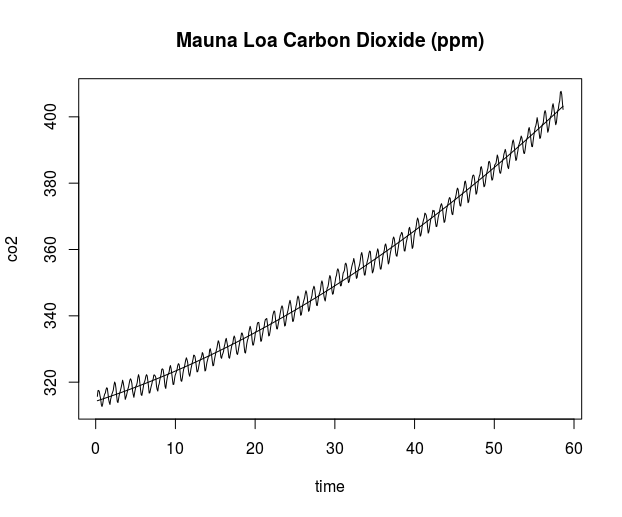
\includegraphics[width=0.7\textwidth, clip]{q1hTime.png} 
	\caption{Quadratic regression of time(with 1958 as origin) and Mauna Loa Carbon Dioxide}
\end{figure}

The quadratic model offers a better fit as compared to the linear model. We can look at the comparisons between predicted start-point/endpoint and actual start-point/endpoint to see that the error has become much smaller. \\

However, the big inherent problem of not being able to take into account of the saw-tooth motion is still present. \\

Although the quadratic model is able to help us reject a linear model, we do not know if the global trend is indeed quadratic-like, or if it is only localized to the 58 years frame.

\subsection{}
 
The standard deviation of the data-misfit residual, or the residual standard error, is 2.21 on 699 degrees of freedom.\\

The significance of the cubic parameter is 0.642, which means that it is not very significant, and the null hypothesis of not having a cubic parameter cannot be rejected.

\section{Fitting Trends and Cycles Over the Entire Data Series}

\subsection{}

The amplitude of the annual cycle in $CO_2$ is $2.833\pm0.06967$ ppm.

\subsection{}

The annual maximum occurs at 0.3095 of the cycle, or approxmiately towards the end of April. A quick sanity check at a zoomed in slice roughly confirms the assertion.

\begin{figure}[htp]
	\centering
	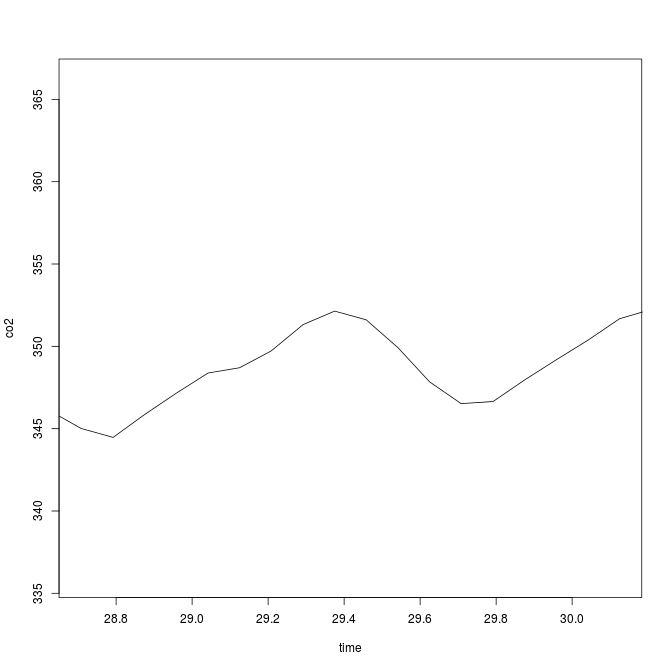
\includegraphics[width=0.7\textwidth, clip]{q2bZoom.png} 
	\caption{Zoomed in slice of time(with 1958 as origin) and Mauna Loa Carbon Dioxide}
\end{figure}
\pagebreak
\subsection{}

\begin{figure}[htp]
	\centering
	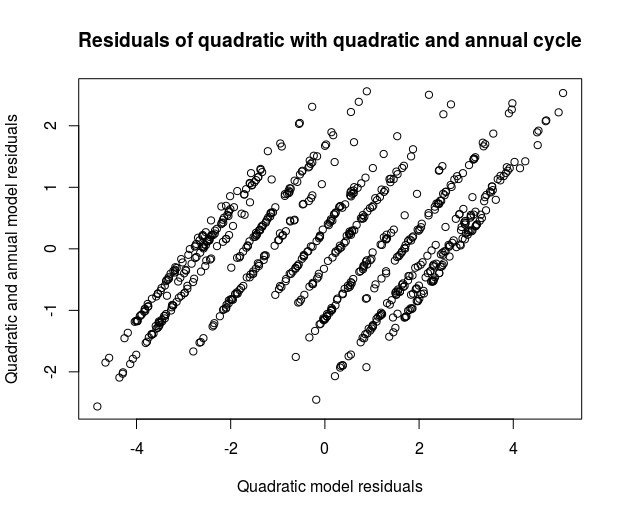
\includegraphics[width=0.7\textwidth, clip]{q2c.png} 
	\caption{Comparing quadratic model residuals with quadratic and annual cycle residuals}
\end{figure}

The standard deviation of the quadratic model only is 2.206 whilst the standard deviation of the quadratic model and annual cycle residuals is 2.064.


































\end{document}